\documentclass{acm_proc_article-sp-sigmod07}

\begin{document}

\title{Framework for comparison between classification algorithms}
\numberofauthors{2}
\author{Luca Gasparella, Enrico Sartori}

\maketitle

\begin{abstract}
This paper presents a framework useful to perform comparisons between
classification algorithms.
The main evaluation measures used are the time used for building the
classification structure, the space consumed by the structure and the
accuracy of the classification provided.

The example provided here is the evaluation of the performances of a
generic decision tree and the Random Decision Tree algorithm by Wei Fan.
\end{abstract}

\section{INTRODUCTION}
The main objective of this work is to measure and compare the performances
of different classification algorithms. In particular we have focused on
the Random Decision Tree algorithm, comparing its performances with a
decision tree based on Information Gain.

During the development of the project we took care of two different
aspects, in fact we provided an implementation of the algorithms tested
and we have implemented a framework able to launch and measure the
performance of the different algorithms.

The evaluation of the algorithm is based on three measures: the time spent
for build the classification structure, the space needed to store and use
this structure and the accuracy of the algorithm.

The accuracy is defined as the percentage of correctly classified
datapoints in a dataset.
For allowing the analysis of the accuracy on every dataset, our framework
integrates the possibility to perform a cross validation over the dataset
using a user chosen percentage of datapoints for training ant the other
for testing.

The testing environment realized permits the setting of many parameters
used for tuning the classification task, in order to measure the influence
of those parameters on the overall performance.

The language chosen for the implementation of the platform and the
algorithms is Python. This choice has been made because of the relative
simplicity of the language which permitted us to focus more attention on
the algorithmic part rather than on solving more fine grain implementation
problems.

In the test section of this work we analyze how the different algorithms
behave when used on different dataset and with different parameters. 

\section{RELATED WORK}

The first algorithm used for comparison is a common Decision Tree, in fact
we wanted to have a comparison of the RDT approach with a commonly used
and known method.
The literature is rich of works about decision tree training and
implementation. In particular \cite{quinlan:induction} gives a complete
background of the basilar techniques used for the realization of such
algorithms.

In this work particular attention is posed into the various measures used
to evaluate the best attribute to use to train the root of a decision
tree.
These techniques are presented in a more concrete way in a tutorial by
Andrew Moore \cite{moore:dtree}. In this presentation the algorithm used is
a decision tree based on information gain as splitting measure, and
presents some ways to optimize and prune the obtained tree.
For the information gain, the same author published a set of slides
in which presents this measure and the way in which it can be computed.

In this work the formal definition of information gain is equation
\ref{infogain}.
\begin{equation}
IG(Y|X) = H(Y) - H(Y|X)
\label{infogain}
\end{equation}
Where Y represent the class and X the attribute tested and the function H
is the entropy.
This function gives a measure of the dispersion of the values in the
dataset.

In particular entropy if an attribute is defined as in equation
\ref{entr}.
\begin{equation}
H(X) = -\sum_{j}^{m} p_j log_2(p_j)
\label{entr}
\end{equation}
Where $p_j$ is defined as $P(X = V_j)$, the probability that X takes value
$V_j$, and $m$ is the number of different values that $X$ admits.

In formula \ref{infogain} appears even the function $H(Y|X)$, defined as
conditional entropy in formula \ref{condentr}.
\begin{equation}
H(Y|X) = \sum_{j} p_j H(X| Y  = V_j)
\label{condentr}
\end{equation}
This value gives the average of the entropy of the attribute $X$ over the
portions of the dataset where $Y$ takes different values.
In fact is the average weighted over the probability of the value $V_j$ of
the specific conditional entropy $H(X| Y  = V_j)$, defined as the entropy
of the attribute $X$ computed among the datapoints where the attribute $Y$
has value $V_j$. 

The second algorithm we choose for the comparison is the Random Decision
Tree presented by Wei Fan in \cite{fan:rdt} which presents the idea to
build a Decision Tree choosing, at each node, an attribute randomly. The
choice is bind on the type of the attribute, in particular if the feature
can assume values in a finite set of options it cannot be chosen again in
the subtree rooted on it. However if the feature is a continuous one, then
a random threshold is choose to split the decision\footnote{The left child
stands for elements that have the value for the attribute less than the
threshold at the node and the right one for the ones which have value
greater or equal than the threshold at the node.} and it can be chosen
again several times in the same subtree accordingly with the ancestor's
decision.

To enhance the accuracy of the method, since the random choice may
leads to different results, multiple trees are trained in order to
approximate the true mean. Considering \emph{k} as the number of features
of the dataset and \emph{N} as the number of trees, then the confidence
probability to have is:
\begin{equation}
\label{formula:confidence}
1 - ( 1 - \frac{1}{k})^N
\end{equation}

Considering the \emph{k} features of the dataset, and the \emph{i}
classifying attributes, the most diversity among trees is with depth of 
\begin{equation}
\label{fig:depth}
\frac{k}{2} 
\end{equation}
since is the maximum value of the combination
\begin{equation}
 {{i}\choose{k}}
\end{equation}

Once the structure is ready the training may take place, in
particular each tuple of the dataset train all the trees generated in
order to read only one time the data. Each node counts how many
numbers of examples go through it.

At the end of the training the leaves contains the probability distribution
of each class, in particular for the tree \emph{i}, considering
\emph{n[y]} the number of instances of class \emph{y} at the node reached
by x, is:
\begin{equation}
\label{formula:probability_tree}
	P_i(\emph{y}|x) = \frac{n[\emph{y}]}{\sum_\emph{y} n[\emph{y}]}
\end{equation}

The classification phase retrieves the probability distribution from each
tree and average on the number of trees generated in the model:
\begin{equation}
\label{formula:probability_forest}
	P(\emph{y}|x) = \frac{1}{N} \sum_{i=1}^N P_i(\emph{y}|x)
\end{equation}


\section{PROBLEM DEFINITION}
The main aim of this work is to produce a comparison between two different
approaches to the classification task. In particular we are focusing our
attention in analyzing the performances of a rather new approach (RDT),
which uses random choices to build the decision tree, and a more common
algorithm based on information gain.

In order do to this we need to provide a reliable implementation of both
the algorithms, which permits us to perform some test and analysis on the
results acquired.

The measures used for comparison are three:
\begin{itemize}
\item The time taken to build the tree and eventually perform the
classification three.
\item The space used to store the tree structure.
\item The accuracy obtained in the classification task.
\end{itemize}

The measure of the space used presented some difficulties, due to the
dynamic typing feature of the language used, in order to solve this we
implemented a method which measures the memory used by an object referring
to the correspondent primitive type of C. This method is explained in
details in following section.

The accuracy can be verified in case of cross validation, classifying a
set of previously known datapoints. This measure can vary depending on the
dataset characteristics. For this reason is important to compare the
results obtained by the two algorithms on the same datasets.

\section{PROPOSED APPROACH}
This section describes and discusses the choice taken during the
development of the project. It will focus first on the implementation of
the platform used for the algorithm comparison and the way it's intended
to be used.
Later the details about the implementation of the algorithms will be
clarified.

\subsection{Classification platform}
This part of the project covers the task of managing the execution of the
algorithms and the measurement of the performances. As for the
classification algorithms, the language chosen for the implementation is
Python, in order to have a more natural interface with the classifier.

The main tasks which this section of the software performs, can be
summarized as follows:
\begin{itemize}
\item Interpret the command line options;
\item Execute the selected algorithm following the options given;
\item Provide support for cross validation;
\item Measure the performance obtained by the algorithm executed;
\item Report the informations retrieved;
\end{itemize}

Before discuss the implementation details is useful give a quick reference
about the usage of the system.

\subsubsection{System usage}
The platform implemented permits the setting of various options, needed
for widen the possibility of performing tests with different algorithms.

The general way in which the system operates is to use a dataset for train
the classifier. Then the platform reads from test dataset and classifies
the datapoints, finally the now classified data are stored in a third
dataset.

The user can specify the attribute to be used as class and a list of
attributes to be ignored in the training task.

One of the most relevant features is the support for cross validation,
with the possibility to select the percentage of data to use for training
and for testing.
When cross validation is enabled is possible to compute a measure of
accuracy of the algorithm. 

Obviously is possible to select the desired algorithm to be used for the
test. In addition to this is possible to choose a particular aspect of the
algorithm itself.

In fact, for the generic Decision Tree is possible to choose the number of
threshold to be tested for the computation of the information gain for
numerical data.
A similar option is usable for the RDT, permitting to set the number of
random tree to be generated.

An outline of the possible options is provided by the following list:
\begin{description}
\item{-t} File containing the training dataset, mandatory
\item{-d} File containing the testing dataset, mandatory if not in cross
validation mode
\item{-o} Output file, mandatory
\item{-a} Name of the class attribute, mandatory
\item{-c} Classifier (classifier\_name[,extra\_parameter]), optional
(generic DT is the default choice), possible names are generalClass or
randomDT
\item{-i} List of ignored attributes, optional
\item{-x} Percentage of splitting for cross validation, optional, enables
cross validation
\end{description}
	
Following the previous outline, an example of usage of the system could be
this example:
\begin{verbatim}
./nukeminer.py -t training.arff -o output.arff \
    -c randomDT,25 -a class -x 60
\end{verbatim}

Launched with this parameters the system executes a cross validation on
the dataset training.arff, classifying on the attribute class. The system
will use the 60\% of the data for training and the 40\% for testing. The
output will be stored in the file output.arff, the algorithm used is the
RDT and will use 25 random trees.

At the end of the execution the system will output the time taken for
train and test the classifier, the memory used to store the data structure
used, and the accuracy reached in this execution.

It's important to notice that the split of the dataset for the cross
validation is performed following a random approach. In this way the
original distribution of the data is preserved in both training and
testing datasets.

This is important to perform a good training of the classifier,
particularly in datasets characterized by having most of the data all in a
single class. This could lead to the situation in which there are no data
belonging to minority class in the training dataset.
Obviously this is a bad situation for training the algorithm.

The technique used by this platform is to scan the dataset and decide for
each datapoint if it belongs to the training or to the testing dataset,
the probability of the outcome of this decision is the one specified by
the user via command line.
This technique assures a more fair division of the dataset.

\subsubsection{File format}
An important remark has to be done for the format of input/output files,
in fact the platform uses a particular file format for handling the data.
It's a simpler version of the ARFF syntax, adapted to fit the needs of the
classification task to be performed.

Is possible to define two types of data: numeric or string. The numeric
type covers both integer and float values, while string is used for
handling categorical data.

For example the following lines represent the header of a dataset file:

\begin{verbatim}
@RELATION iris

@ATTRIBUTE sepallength	numeric
@ATTRIBUTE sepalwidth 	numeric
@ATTRIBUTE petallength 	numeric
@ATTRIBUTE petalwidth	numeric
@ATTRIBUTE class string 

@DATA
\end{verbatim}

This is the adapted header of the Iris dataset, after the keyword DATA
is possible to write the tuples, as a list of values separated by a ','
character, as in the following example:

\begin{verbatim}
@DATA
5.1,3.5,1.4,0.2,Iris-setosa
4.9,3.0,1.4,0.2,Iris-setosa
4.7,3.2,1.3,0.2,Iris-setosa
\end{verbatim}

\subsubsection{Performance evaluation}
The main objective of the platform is to provide a system able to measure
the performance of a particular algorithm completing the task assigned.
As said in the introduction the system bases the evaluation on three main
measures: time, space and accuracy of the classification.

The classification process goes through two main phases, the first one,
the most long and difficult, is the construction of the decision tree,
while the classification of unknown datapoints is generally a less
demanding operation.

The platform presented here can evaluate the time needed both for
constructing the tree and for classifying a test dataset. 
Even if the time needed for classifying a dataset is often a fraction of
the time used for building the tree, the behaviour of different algorithms
on this operation can be very important.

An example of the importance of this value can be represented by the case
of an on-line classifier. In this particular environment the time needed
for classify a datapoint is a vital parameter for the evaluation of the
performance of the algorithm.

The technique used for evaluate the time spent on the whole classification
task is fairly simple. In fact the platform simply measures the time
elapsed between the start and the end of the process.

Besides its simplicity and robustness, this approach presents some
drawbacks. The main is that this way of measuring time performance is
strictly dependent on the machine used for executing the test.
Therefore in order to retrieve reliable result from a comparison between
two algorithms is better to execute them on the same machine.

Another problem is represented by the possibility of interferences from
other programs and daemons running on the machine. These interferences can
lead to a drop of performances in term of time.

An alternative way of counting the time spent for the execution of the
algorithm could be use, instead of the second elapsed, the clock cycles
used by the program. 
This measure unit would be less immediate to understand and less natural.

During the development of the project has been preferred to use seconds as
the measure unit, taking care of execute the program in controlled
environment on a dedicated machine.

The measure of the space is equally important, in fact the dimension of
the dataset to analyze can be very huge, or theoretically infinite, as in
the case of many application of online classifiers.
This shows the importance of the measure of the space used for running the
classification algorithm, the risk is to build a structure which cannot
fit in the main memory of the machine used.

For the algorithms implemented for this comparison, this case has not been
considered, considering valid the assumption that the dataset can always
fit in main memory.
The reason of this choice is that implement some ways to reduce the
footprint in memory of the structure used, maybe storing some less used
branches of the tree on disk, could be very difficult to be realized in
equal way between the two algorithms.

The differences between the structures used in the two algorithms, are too
relevant to assume that the same time will be spent in storing and reading
the cached data from disk. These difference will corrupt the results in
time evaluation.

Moreover, avoiding the usage of caching techniques, is possible to
retrieve a detailed picture of the actual memory usage of the algorithm at
any time. 

Another remark about measuring the memory used by the structure regards
the language used for the implementation.
In fact Python features dynamic typing, this poses difficulties in the
evaluation of the actual amount of memory used to store a
particular object.

For dealing with this issue,the memory used by an object is computed using
the size of the C primitives types corresponding to the Python types used.

The last measure considered for evaluate the performances of the
algorithm is the quality, or accuracy, of the classification performed. 
This measure is very indicative in particular if compared with the time
measure.
In fact often, in many problems of computer science, the solution of a
problem is a balance of the trade-off between time and quality.

In the platform presented here the computation of the quality of the
classification obtained is possible only when the system runs in cross
validation mode. In fact, when performing this kind of test, is sure that
even the testing dataset contains the correct classification.

Therefore is easy to compare the classification computed by the algorithm
with the real values in the dataset.
The system finally computes the percentage of correctly classified
datapoints over the size of the testing dataset.
This value is considered the measure of the quality of the classification
obtained.

A possible drawback of this approach is represented by the particular
situation in which a very large majority of the training datapoints
belongs to the same class.
The building of the decision tree, therefore, will be based on a large
amount of informations from the largest class, while the other will be
less represented in the final tree.

A direct consequence of this is that the classifier will choose as class
the major one more likely, generating many misclassifications for the
least relevant class.

The level of accuracy, anyway, will remain quite high, this because the
large even in the test dataset the large majority of the data will belong
to the most probable class. The elements in the least relevant class are
so few that, even if most of them are not correctly classified, the
accuracy level doesn't reflect this situation.

\subsubsection{Reporting}
The last task for the platform is to output some form of report
illustrating the result obtained from an experiment.
The method chosen for this platform is to implement a BASH script that
manages the execution of the two algorithms several times with different
parameter on a dataset.

This script reads the output of the program and collect the useful data,
writing the results in a format usable with the utility gnuplot for being
transfered into charts.

This method provides a simple way to have an intuitive comparison between the
results of the two different algorithms.

Once the script ends its cycle, the local directory ``plot'' will contain
five graphs: accuracy.ps, training.ps, classification.ps, nodes.ps and
memory.ps. The syntax of the tool is:
\begin{verbatim}
./evaluation.sh <dataset> <classification attribute>\
     [<ignore attribute> <ignore attribute>]\
     [--trees=<number>] [--thresholds=<number>]
\end{verbatim}

An example of use is the following:
\begin{verbatim}
./evaluation.sh iris.arff class sepallength\
   --trees=5 --thresholds=3
\end{verbatim}

The script will execute both algorithms on the input dataset cross
validated starting from 1\% to 100\% with step of ten percent classifying
with respect to the attribute ``class'' and ignoring attribute
``sepallength''. The parameter ``trees'' explicits the number of tree to be
generated by the RDT algorithm, whereas the ``thresholds'' parameter
explicits how many test must be done in the Decision Tree algorithm for
each node.

\subsection{Decision Tree}
The first algorithm considered for the comparison is a generic Decision
Tree. Has been chosen because it's a well known approach and is a good
base for a comparison with another algorithm.

The measure chosen for selecting the attribute on which split the dataset
is the information gain.
The computation of this measure on categorical values is quite a simple
operation. When considering numerical values the situation changes, in
fact considering the specific conditional entropy for every possible value
assumed by a numerical attribute is a waste of resource and won't give
reliable results.

A different approach, followed in this implementation of the algorithm, is
to compute the information gain of a threshold on which split the dataset.
In this way a node is split in two children, one containing the data with
the chosen attribute less than the selected threshold and the other
containing the rest 

To perform the computation of the information gain, the algorithms splits
recursively the dataset owned by the node. 
This operation is performed until is possible to compute the specific
conditional entropy for the label with respect to each different attribute
and its values.

For the numeric values a similar behaviour is adopted, but, instead of
splitting the dataset with respect to each different value of the
attribute analyzed, the split is performed using a threshold.

Another important operation to be performed before training a node is to
select a set of candidate threshold for the numeric attributes, on which
compute the information gain, and eventually split the node.
In order to perform this task the algorithm sorts the values of the
selected attributes and bucketizes it, following a equi-depth approach.

Besides the cost in time for sorting the list of values, which is $n log
n$ in the worst case (using the built in python implementation), this
approach offers a more sharp way for threshold selection, than through a
sample of the dataset.

\subsection{Random Decision Tree}
In the first implementation of the algorithm, that was rigorous to the
pseudocode presented in \cite{fan:rdt} that is build the tree before the
training, testing with a dataset having different discrete feature, such
``Adult'', the tree generated was very big and the time to construct it was
very expensive; in particular, building a tree having depth equals to the
number of attributes, instead of the half, the Python interpreter
aborted its execution due to memory problems.\footnote{In the test we
conducted on a training dataset with 13 attributes, nine of them with
more than six possible values, and 26065 elements, the number of node for
the tree with depth 13 was over one million.}
The tree presented by the pseudocode is the one with all possible values
that features may assume but it can be rather empty once it has been
trained in the case there are a lot of discrete features . Some tests
on different datasets reveal that is not useful to produce a bigger tree if
data can not fit it.

In order to solve the problem the tree's building phase has been merged
with the training phase and nodes are generated only if there is an element
that can go through them. This lead to a compact tree where
each node is crossed by at least one element.\footnote{With the same
conditions as before, now the algorithm performs the train generating a
tree with at least 4060 nodes.}

If the training dataset is not expressive on the possible values
the attribute can assume, the trained tree may be less accurate.
Accordingly with the confidence in \ref{formula:confidence} the inverse
formula
\begin{equation}
\label{formula:N_generate}
N = \log_{1-\frac{1}{k}}({1 - \emph{confidence}})
\end{equation}
allows to calculate the numbers of tree to generate in a dynamic way. In
 particular if the number of examples to train the model is less than
2000\footnote{Experimental tests conducted by Wei Fan show that this
examples history is generally enough to have a good confidence even with a
low number of tree generated.} the \emph{confidence} is set to 95\%,
whereas if it is greater is set to 70\%. The tests conducted in all the
datasets show the efficiency of the method in analyzed that improve the
timing without any accuracy loss.

The algorithm is contained in the ``randomDT.py'' Python file and consists
of four classes. The main one is ``Classifier'' that allows to interface
with the support class ``class\_mgr.py'' through the three default methods
``train()'', ``classify()'' and ``get\_memory()''. Moreover the class is
charged to remove the attributes to ignore and to perform the
classification.

The ``Forest'' class is a virtual representation of the set of trees
generated. In particular the function ``best\_forest()'' configure the
number of trees to generate accordingly with \ref{formula:N_generate}
speeding up the execution, but maintaining the accuracy.

The ``RandomDT'' class represent the Random Decision Tree, in particular
in the initialization, if is requested a simple node, then a random
element from the list of attributes given as parameter is chosen and the
ranges, the second parameter, is on purpose modified: if the attribute is
continuous then a random threshold is chosen accordingly with
ranges and two sons are generated, whereas in the case of a discrete
feature, ``threshold'' will contain the possible values it can
assume, coming from ranges from which will be deleted to avoid a choice
in the subtree, and will be used to indexed the ``children'' field.
The class offers also the method to retrieve the probability distribution
as in \ref{formula:probability_tree} from the tree given the tuple to
classify.

The ``Trainer'' class aims to build and train the entire forest of RDTs.
In particular the procedure ``build\_train()'' manages the retrieving and
updating of the forest calling the recursive procedure
``tree\_updating()'' which performs the building of the tree, updating the
existing nodes. The latter procedure take distinction in generation about
the two kind of foreseen attributes resulting the bigger slice of code in
the algorithm.

\section{Experimental Evaluation}
The tests have been conducted on two different machines, but same
architecture, and no relevant differences were observed. The datasets
considered are not equally populated by the two kind of attributes
foreseen and they may be not real ``representative'' of the distribution.

In order to compare the two algorithms the ``Adult'' dataset was taken as
primary check since it contains different kind of attributes and it is
quite big. In particular the dataset present fifteen attributes, nine of
them of string type, and classify over a string attribute, ``gain'',
ignoring two numeric features, ``fnlwgt'' and ``education-num''. The
command executed is:
\begin{verbatim}
./evaluation.sh adult.arff gain fnlwgt education-num
\end{verbatim}

Another interesting dataset used is the ``Xenon'', this dastaset contains
samples of the concentration of four isotopes of the Xenon in the
atmosphere. The dataset is divided into two classes, which say if the
concentration levels are normal or the footprint of a nuclear weapon test.
This dataset permits to evaluate the algorithms behaviour on numeric
values.

In figure \ref{fig:adult_standard} are shown all the output graphs
obtained.  For a better comparison with Decision Tree the number of nodes
for RDT algorithm is referred to a single tree, randomly chosen among the
others.
The \ref{fig:depth} assure a good reduction in terms of nodes and the
choice has a direct results on the graph about the number of nodes
generated.

The memory usage for the RDT is very high due to implementation that was
focused on the comprehension rather the efficiency in order to simplify
the readability. The huge employment comes from the storing of the
values of the discrete features in the nodes to index the children. Since
there are several trees this facilitation exploits with the number. In the
test there was built sixteen trees, so the space allocation for a single
tree, for the maximum case, is:
$$ \frac{3500000}{16} Byte = 218750 Byte$$
And so the single tree is proportional to the one built by the Decision
Tree. The non-linear trend of the graph is due to the different tree
structure generated at each step. Since the attribute to test in the node
is purely a random choice it may happens that one of the nodes near to
root is a discrete feature with a lot of sons and so the entire tree is
conditioned by the choice.

The number of trees has impact also in the training time and the
classification time, of course. In particular for train a tuple the RDT
algorithm spend on average 6.5\emph{ns} whereas to classify a tuple it
spends on average 5.6\emph{ns}. It is rather efficient, but considering
the whole forest of tree the time acquire a significant value. Considering
the test, the number of tuples trained are about 26000, whereas the tuples
to classify are around 6500:
$$
26000 * 6.5\emph{ns} * 16 \sim 27 s
$$
$$
 6500 * 5.6\emph{ns} * 16 \sim 5.8 s
$$

About the accuracy the RDT algorithm shows a stable accuracy, little
better than the Decision algorithm.

\begin{figure*}
\label{fig:adult_standard}
\centering
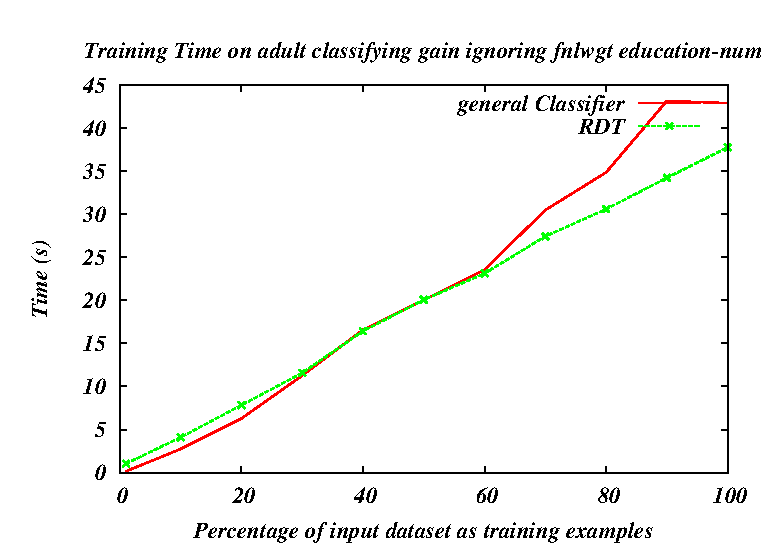
\epsfig{file=training.ps,scale=0.60}
\epsfig{file=classification.ps,scale=0.60}
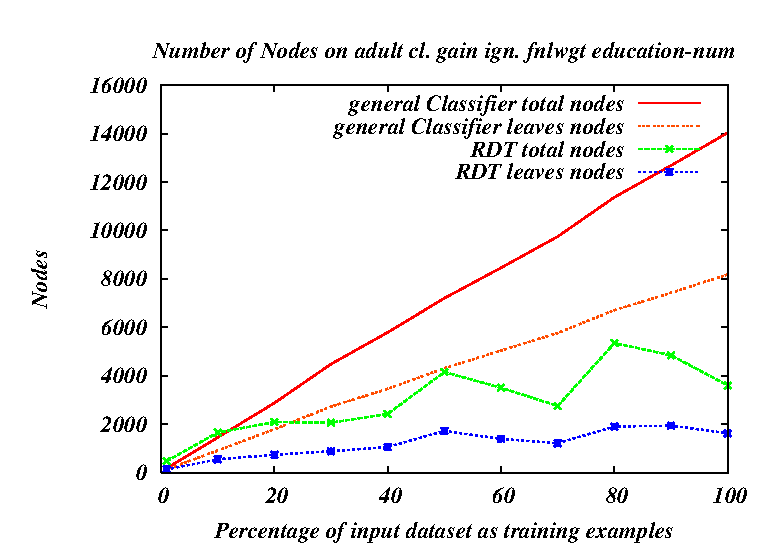
\epsfig{file=nodes.ps,scale=0.60}
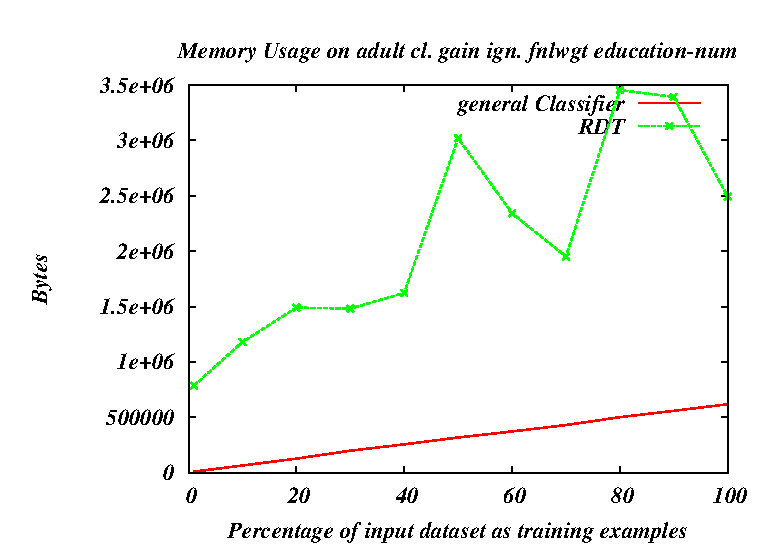
\epsfig{file=memory.ps,scale=0.60}
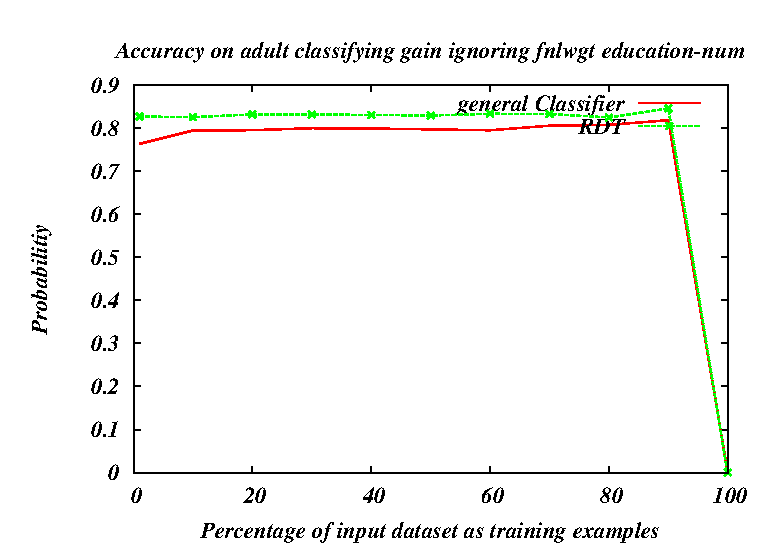
\epsfig{file=accuracy.ps,scale=0.60}
\caption{Running the framework on the Adult dataset classifying over gain
and ignoring the attributes: fnlwgt and education-num.}
\end{figure*}

\begin{figure}
\label{fig:adult-50}
\centering
\epsfig{file=training_adult-50.ps,scale=0.60}
\epsfig{file=nodes_adult-50.ps,scale=0.60}
\epsfig{file=accuracy_adult-50.ps,scale=0.60}
\caption{Running the framework on the Adult dataset classifying over gain
and ignoring the attributes: fnlwgt and education-num with 50 trees.}
\end{figure}

\begin{figure}
\label{fig:adult-occupation}
\centering
\epsfig{file=training_adult-occupation.ps,scale=0.60}
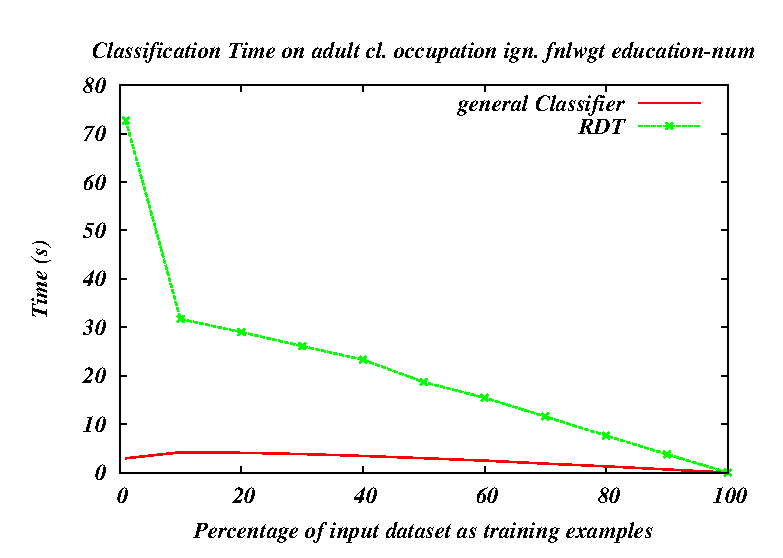
\epsfig{file=classification_adult-occupation.ps,scale=0.60}
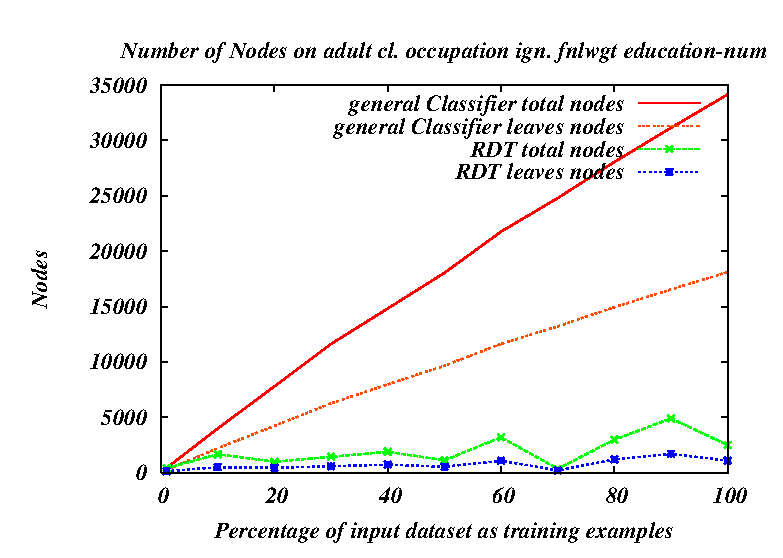
\epsfig{file=nodes_adult-occupation.ps,scale=0.60}
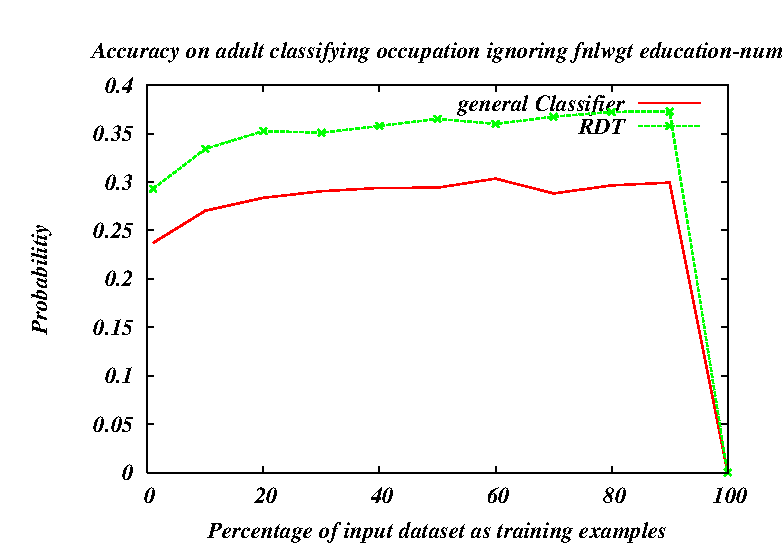
\epsfig{file=accuracy_adult-occupation.ps,scale=0.60}
\caption{Running the framework on the Adult dataset classifying over
occupation and ignoring the attributes: fnlwgt and education-num.}
\end{figure}

\subsection{Improvements}
There are some improvements that the framework can be submitted.
The Decision Tree algorithm may be enriched with the possibility to
calculate also the Gini Index and can be left to user the choice to use 
one or the other. 
For the RDT algorithm may be improved in particular the Memory usage. At
the moment each value that a discrete feature may assume is stored in the
node growing its dimension. A possible easy solution is to index the child
as the order of possible values are passed to the software. The advantage
in memory consumption is considerable.

Another feature to enrich the framework is the option to save the model
and reload in order to facilitate the study with a bigger structure. In
the case the Python module ``Pickle'' allows to serialize and de-serialize
Python object structures converting it in a Byte stream.

The script may be optimized to perform the management of an arbitrary
number of algorithm and more parameter should be acquired through it.

\section{Conclusions}
The two algorithms both generate the tree in a similar way and the tests
conducted on the datasets considered, reveal the efficiency of the solution
based on the Probability Theory, but without a greater advantage in the
average. The Random Decision Tree doesn't need particular additional
calculus except for some simple comparison, whereas the Decision Tree
founds its job on the Information Gain that require more time.

As confirmed by the tests performed, the number of trees generated in RDT
influences deeply the time performance of the algorithm. For this reason
the solution implemented for selecting dynamically this value confirms to
be an important improvement for this algorithm.
\bibliographystyle{abbrv}
\bibliography{report}
\end{document}
